\documentclass[12pt]{article}

\usepackage[portuguese]{babel}
\usepackage{float}
\usepackage{listings}
\usepackage{indentfirst}
\usepackage{amsfonts, amssymb, amsmath}
\usepackage{graphicx}
\usepackage{enumitem}
\usepackage[colorlinks=true, allcolors=blue]{hyperref}
\usepackage[letterpaper,
            top=1.5cm,
            bottom=1.5cm,
            left=2.75cm,
            right=2.75cm,
            marginparwidth=1.75cm]{geometry}

\title{Lista 3 -- AFD, AFND, Transformação AFND - AFD, Minimização}
\author{Guilherme Lopes}
\date{\today}

\begin{document}
\maketitle

    % \begin{itemize}[label=R:]
    %     \item 
    % \end{itemize}

\begin{enumerate}
    \item Desenvolva automatos que reconhecam as seguintes linguagens:
    \begin{enumerate}[label=\alph*)]
        \item $\{w\in{a,b}^*| aaa \text{ é subpalavra de } w\}$
        \begin{itemize}[label=R:]
            \item 
        \end{itemize}
        \item $\{w\in{a,b}^*| \text{O sufixo de } w \text{ é } aa\}$
        \begin{itemize}[label=R:]
            \item 
        \end{itemize}
        \item $\{w\in{a,b}^*| w$ possui uma quantidade par de $a$ e impar de $b$ 
        ou quantidade impar de $a$ e par de $b\}$
        \begin{itemize}[label=R:]
            \item 
        \end{itemize}
        \item $\{w\in{a,b}^*|$o quinto simbolo da direita para a esquerda de $w$ 
        é $a\}$
        \begin{itemize}[label=R:]
            \item 
        \end{itemize}
    \end{enumerate}
    \item A partir dos AFNDs para as linguagebs descritas nos itens $a$ e $b$ 
    do exercicio anterior, descreva AFDs (mostrando o processo de transformação) 
    e encontre os automatos minimos para os mesmos.
    \begin{enumerate} [label=\alph*)]
        \item \
        \begin{figure}[H]
            \centering
            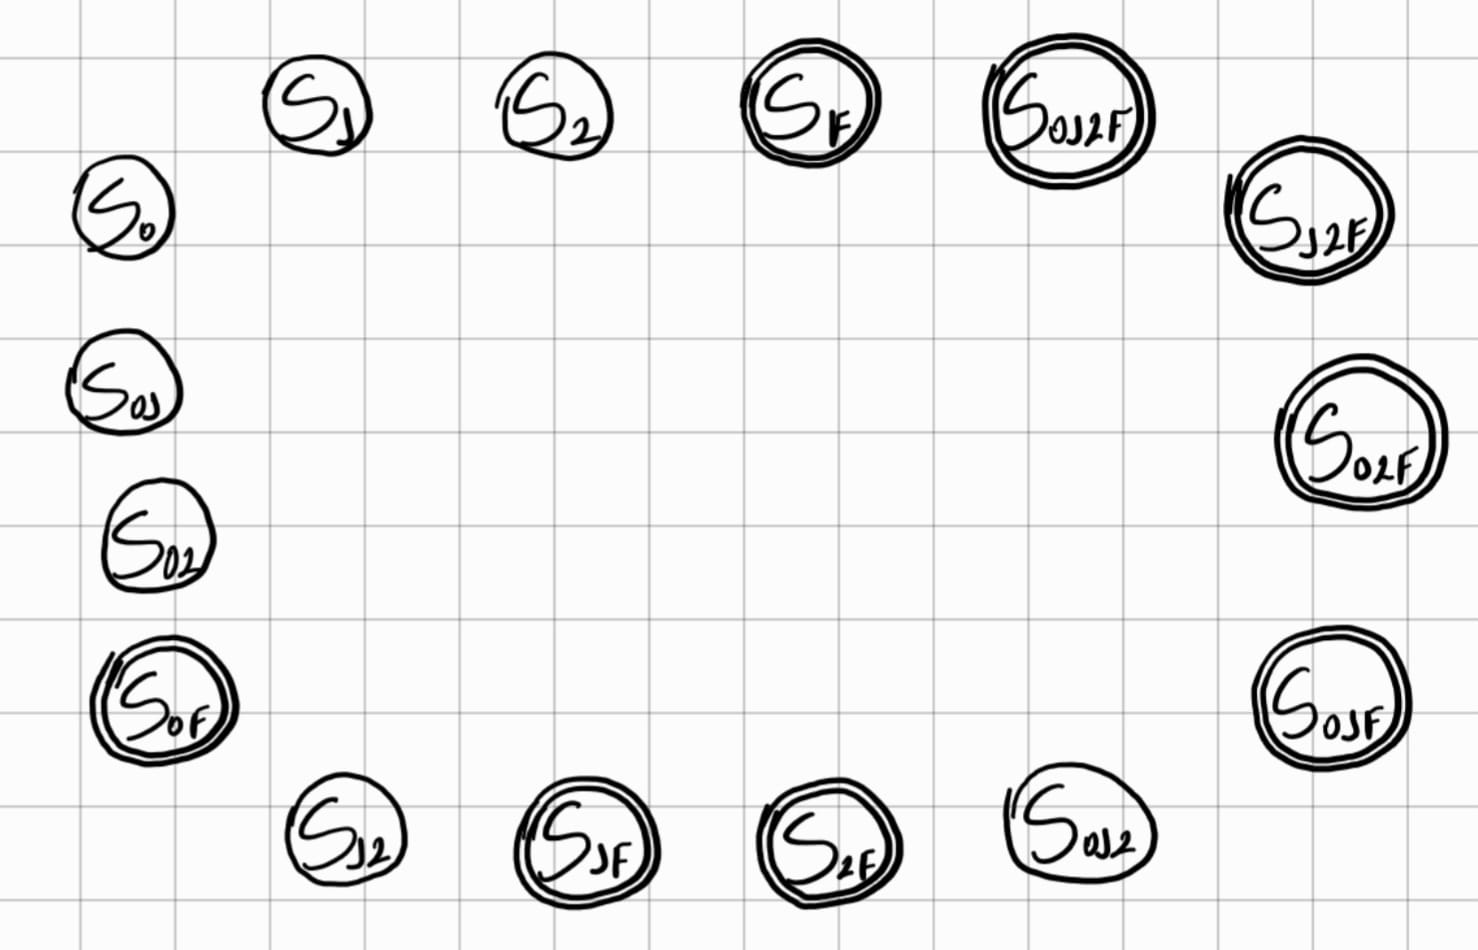
\includegraphics[width=0.6\linewidth]{imagens/ex5a/ex5a1.jpeg}
            \caption{Definido as combinações possiveis de estado}
        \end{figure}
        \begin{figure}[H]
            \centering
            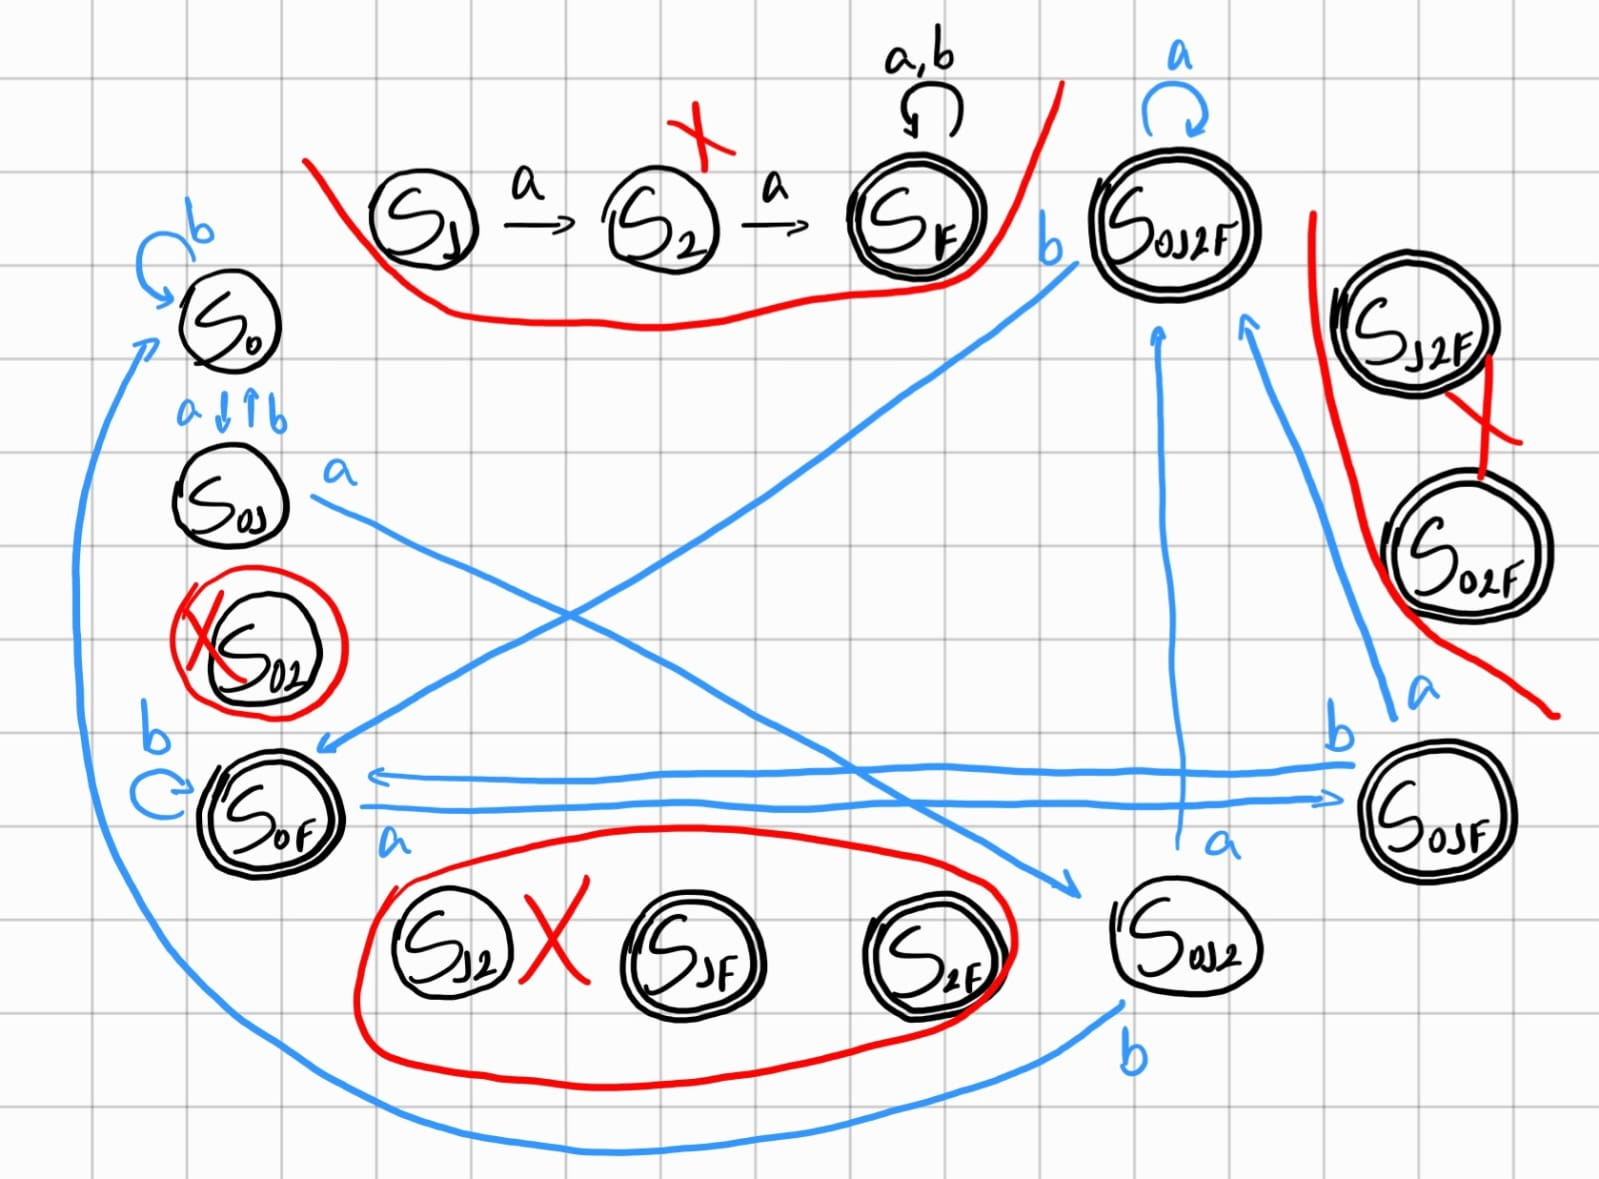
\includegraphics[width=0.6\linewidth]{imagens/ex5a/ex5a2.jpeg}
            \caption{Criado as transições e excluido os estados não utilizados}
            \vspace{16pt}
            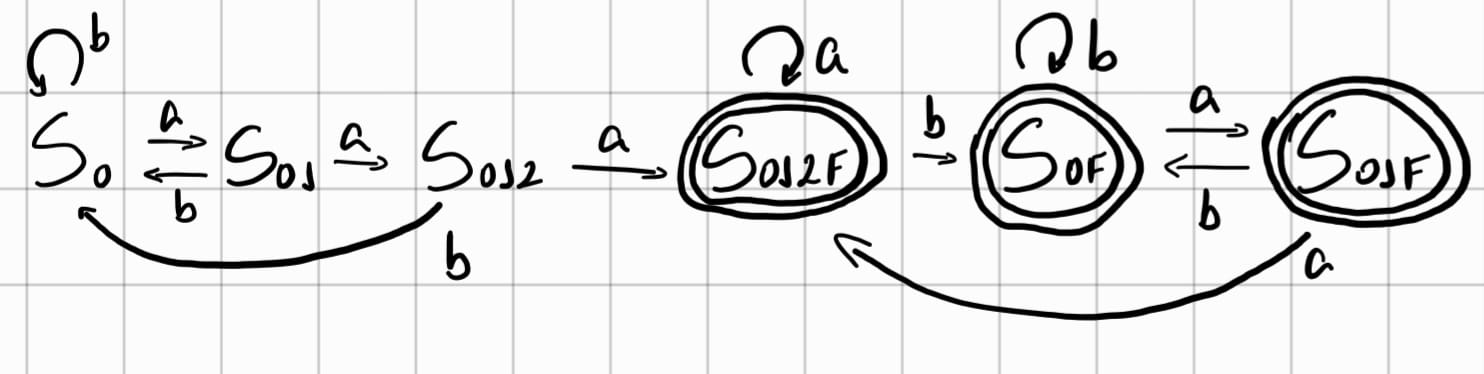
\includegraphics[width=0.7\linewidth]{imagens/ex5a/ex5a3.jpeg}
            \caption{Organizado os estados para ficar mais visivel}
            \vspace{16pt}
            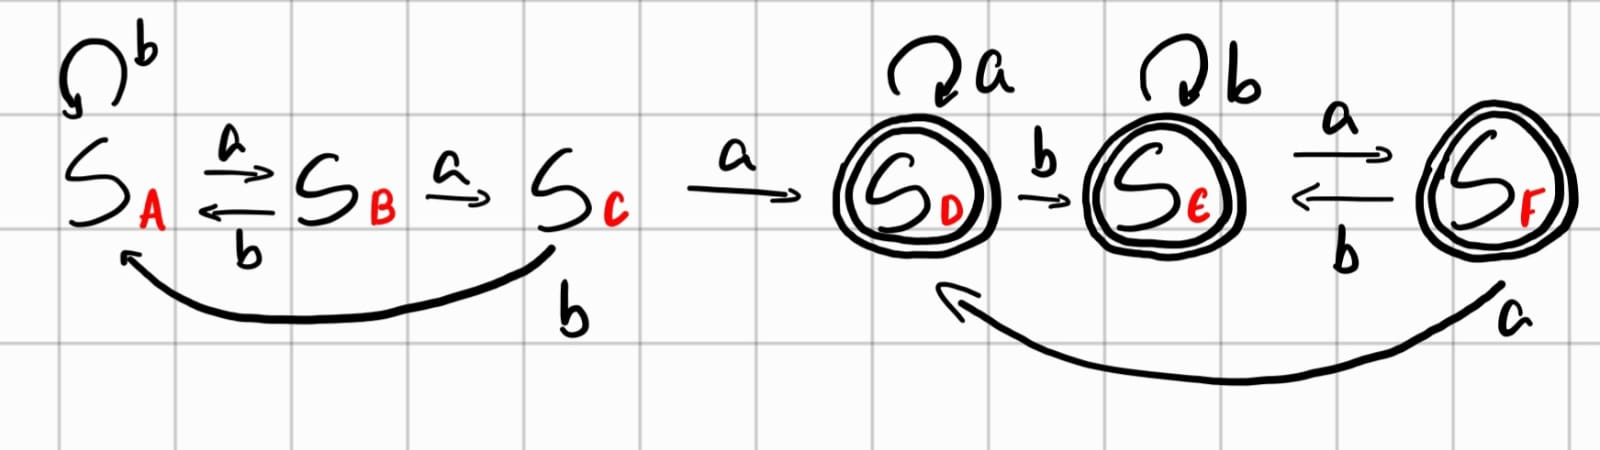
\includegraphics[width=0.7\linewidth]{imagens/ex5a/ex5a4.jpeg}
            \caption{Renomeei os estados para ficar mais fácil de entender e 
            ajuda na minimização}
            \vspace{16pt}
            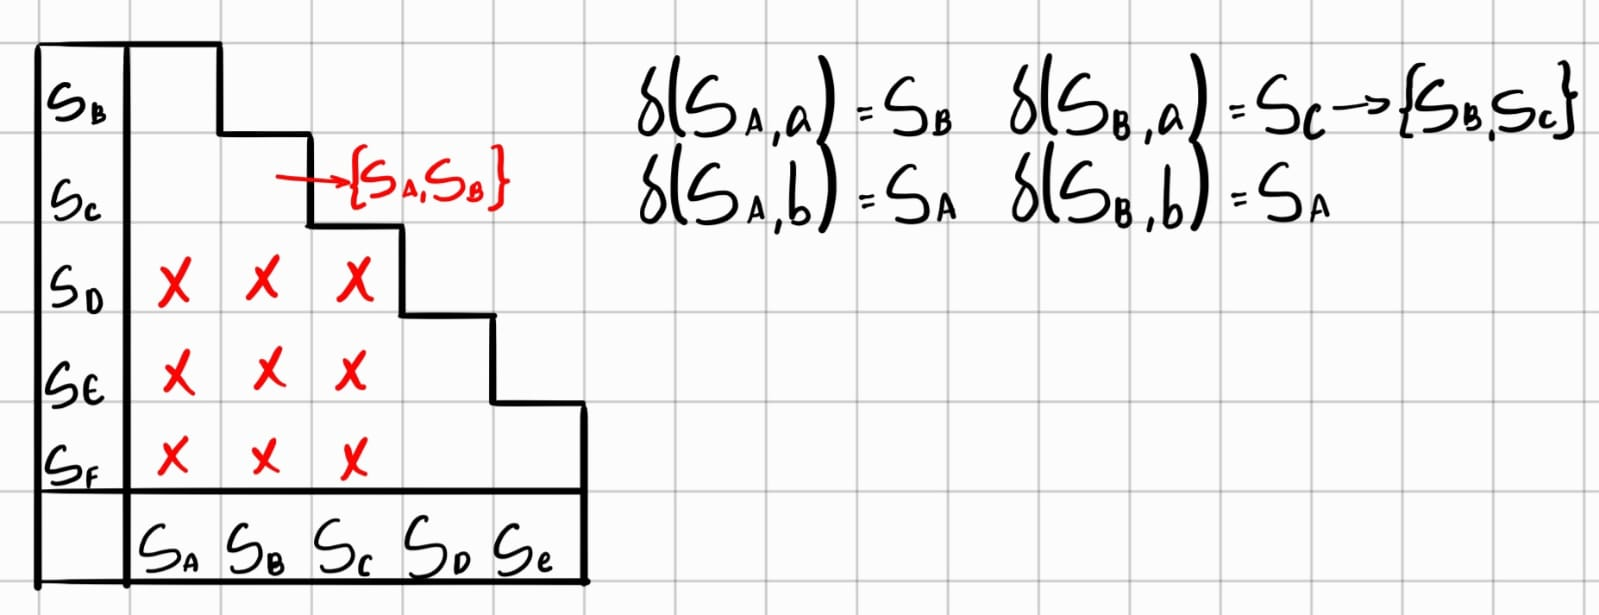
\includegraphics[width=0.7\linewidth]{imagens/ex5a/ex5a5.jpeg}
            \caption{Tabela de minimização começando com $\{S_A,S_B\}$}
        \end{figure}
        \begin{figure}[H]
            \centering
            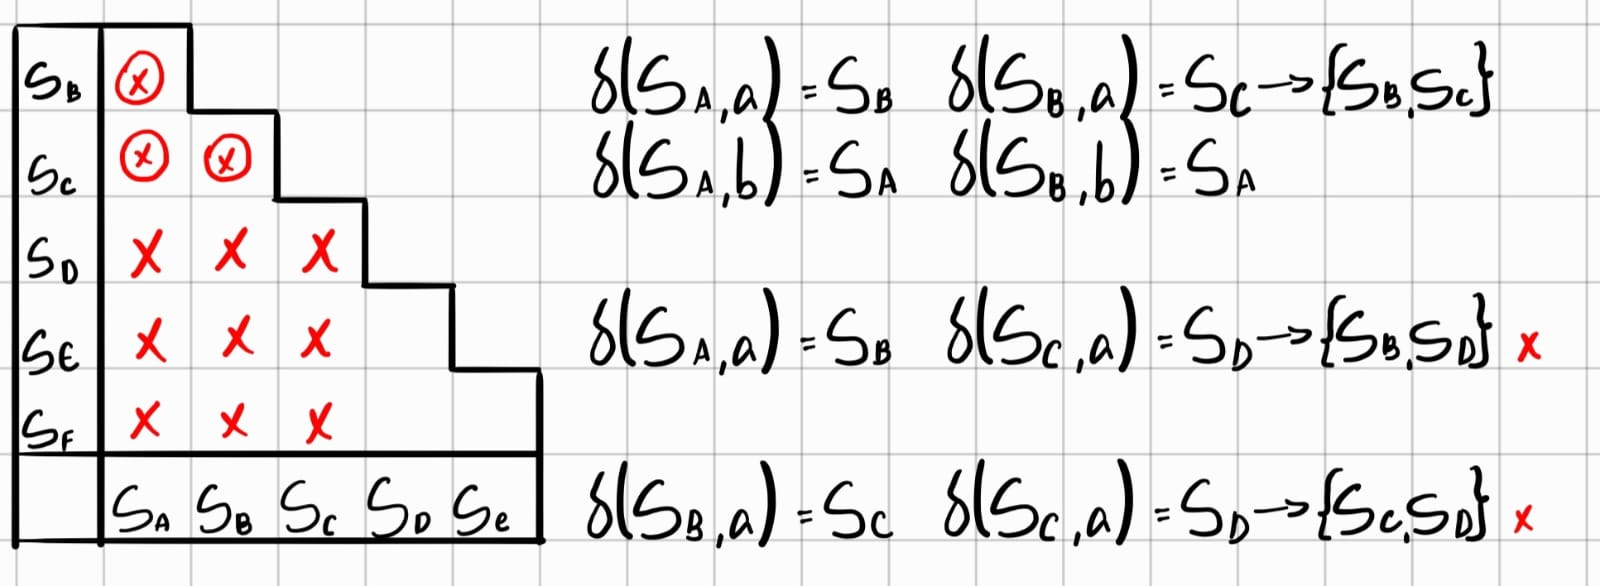
\includegraphics[width=0.7\linewidth]{imagens/ex5a/ex5a6.jpeg}
            \caption{Ao fazer $\{S_A,S_C\}$ e $\{S_B,S_C\}$, concluimos que não 
            se equivalem}
            \vspace{16pt}
            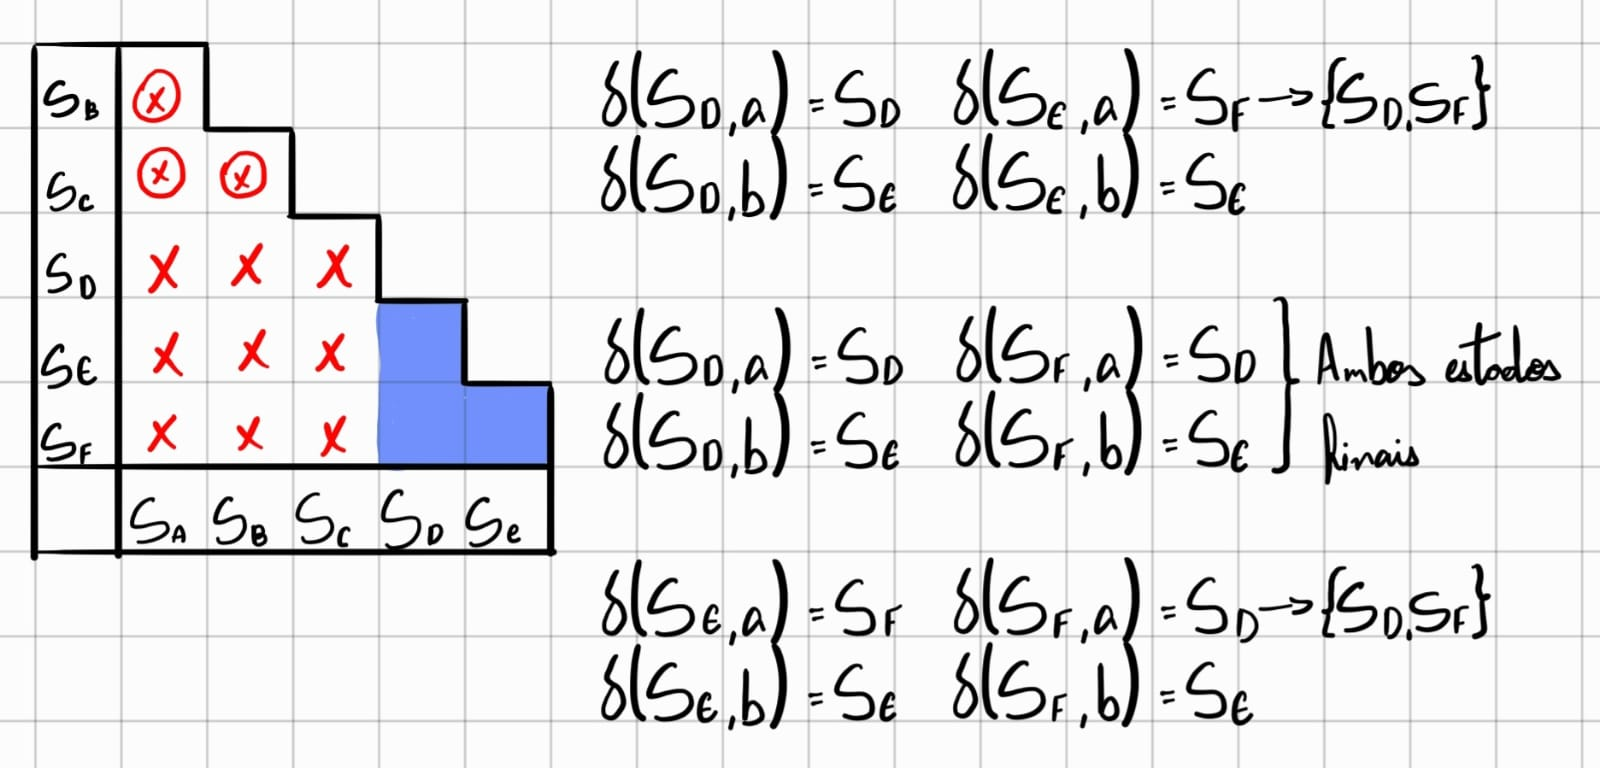
\includegraphics[width=0.7\linewidth]{imagens/ex5a/ex5a7.jpeg}
            \caption{Definimos que $\{S_D,S_E,S_F\}$ são equivalentes}
            \vspace{16pt}
            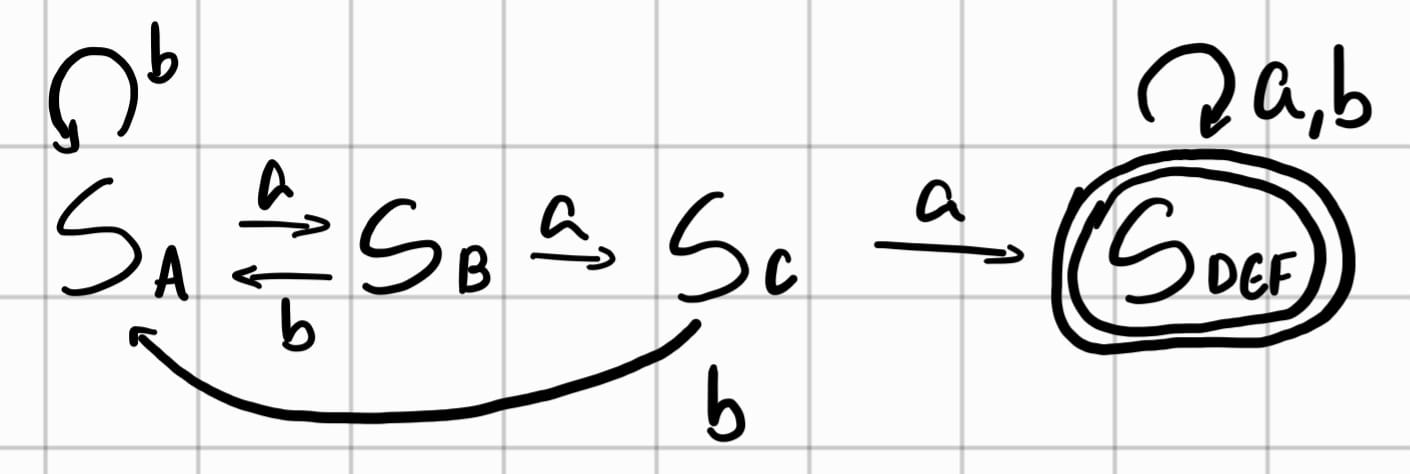
\includegraphics[width=0.7\linewidth]{imagens/ex5a/ex5a8.jpeg}
            \caption{AFD minimizado!}
        \end{figure}
        \vspace{7cm}
        \item \
        \begin{figure}[H]
            \centering
            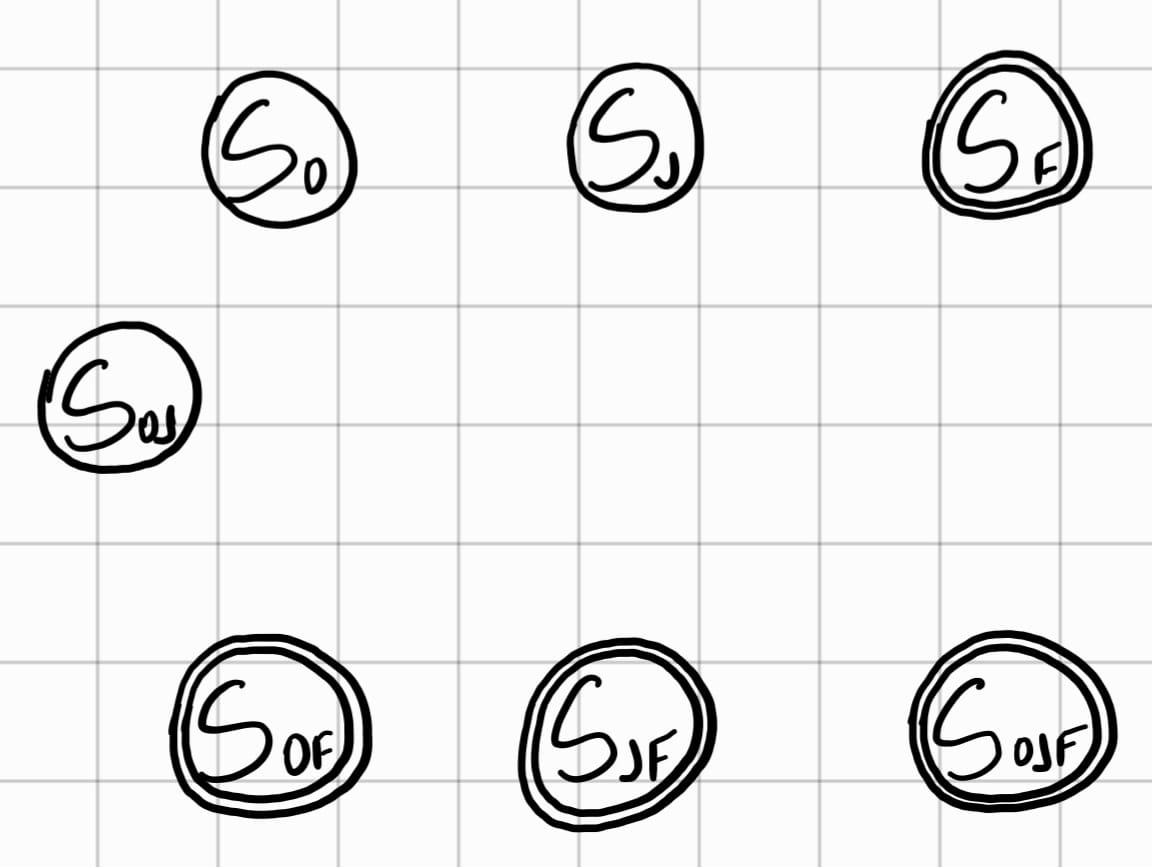
\includegraphics[width=0.6\linewidth]{imagens/ex5b/ex5b1.jpeg}
            \caption{Definido as combinações de estado}
            \vspace{16pt}
            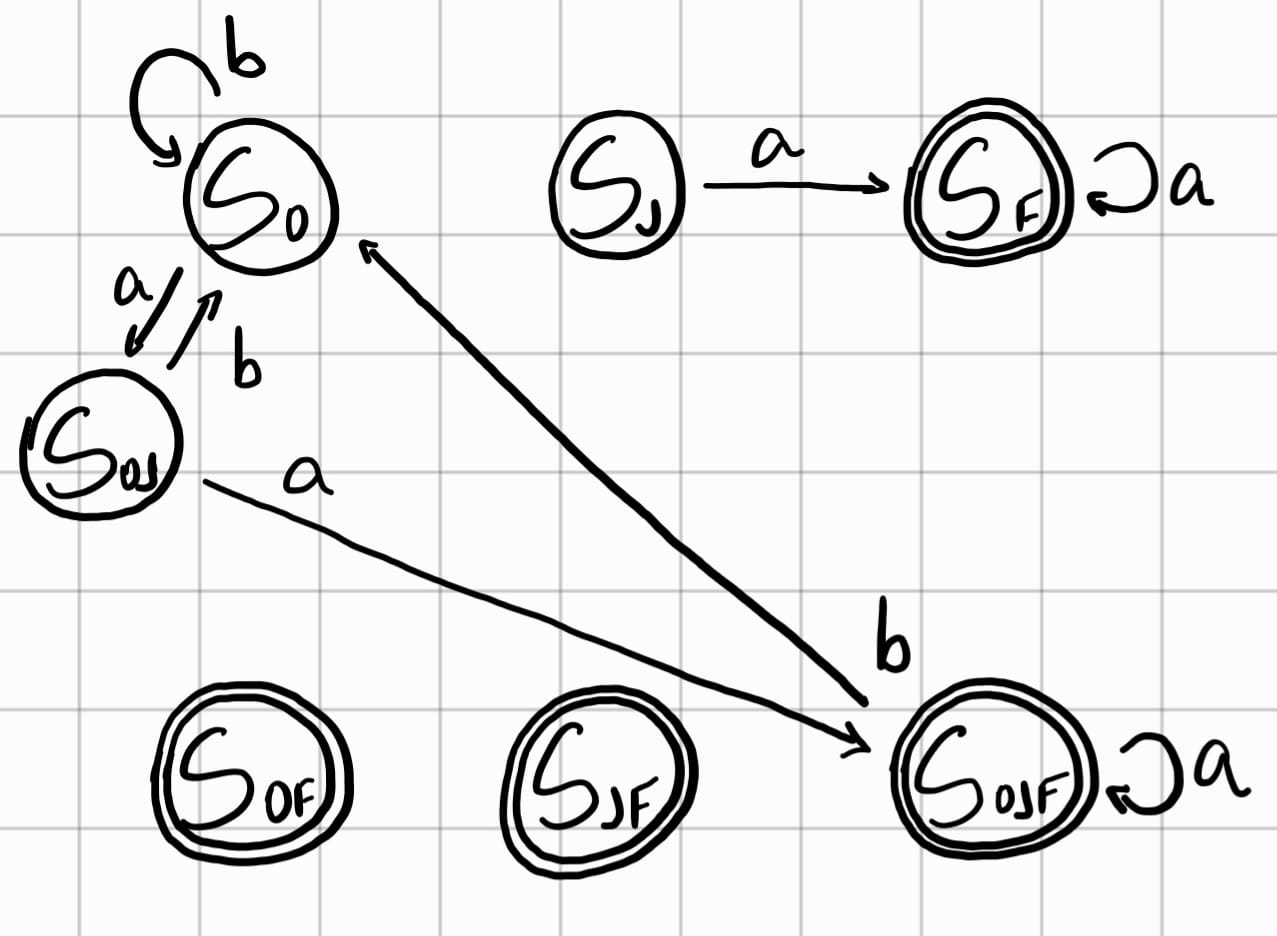
\includegraphics[width=0.6\linewidth]{imagens/ex5b/ex5b2.jpeg}
            \caption{Criado as transições de estado}
            \vspace{16pt}
            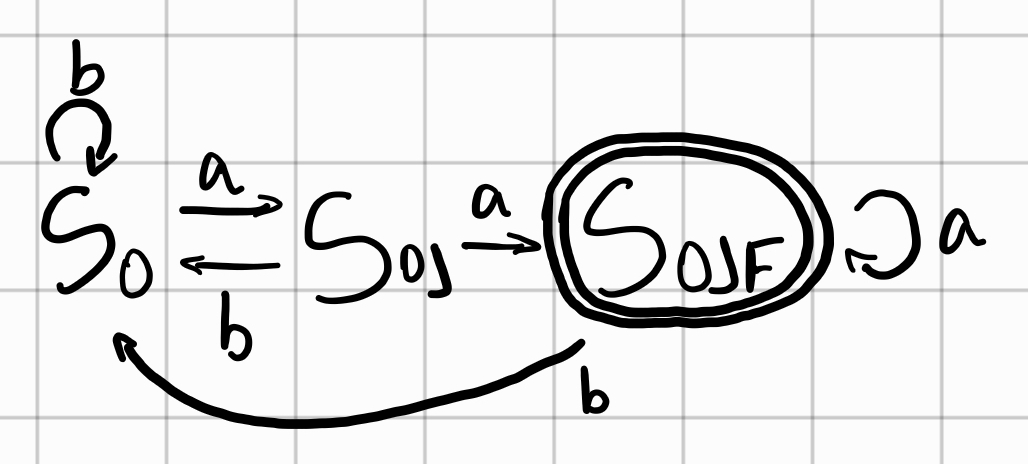
\includegraphics[width=0.6\linewidth]{imagens/ex5b/ex5b3.jpeg}
            \caption{AFD minimizado}
        \end{figure}
    \end{enumerate}
    \vspace{0.5cm}
    \item Minimize os autômatos mostrados nos diagramas a seguir
    \begin{enumerate}[label=\alph*)]
        \item 
    \end{enumerate}
\end{enumerate}

\end{document}